\section{Results}\label{model.res}
This section presents the results of model calibration, including:
the posterior distributions of calibrated parameters (see Table~\ref{tab:par.defs} for definitions),
and the modelled patterns of transmission among risk groups in Eswatini over time.
%===================================================================================================
\subsection{Posterior Parameter Distributions}\label{model.res.par}
Figure~\ref{fig:post.distr} illustrates the distributions of calibrated model parameters,
stratified by prior (all samples) \vs posterior (top 1\% by calibration likelihood).
Many of the distributions do not significantly differ
(Anderson-Darling Test \cite{Scholz1987}),
indicating that calibration did not reduce uncertainty in these parameters.
While more advanced model calibration techniques
might improve parameter inference \cite{Menzies2017},
the overall model fit was judged to be sufficient
for the downstream research questions (\ie \sref{intro.rqs}).
A total of 20 parameters had highly significant differences ($p < 10^{-5}$)
between prior and posterior distributions:
% MAN
\begin{itemize}
  \item \textbf{Mean increased:} \foreach \pp in \ppincr{\texttt{\pp}, }
  \item \textbf{Mean decreased:} \foreach \pp in \ppdecr{\texttt{\pp}, }
\end{itemize}
Such differences overwhelmingly tended towards increasing overall HIV transmission,
suggesting that the set of prior distributions tended to underestimate transmission risk,
despite several adjustments towards increasing transmission risk (\sref{model.par}).
Indeed, the high HIV prevalence in Eswatini, and other generalized epidemics,
has long been challenging to explain based on the available data \cite{Whiteside2003,Shelton2010}.
\begin{figure}
  \centering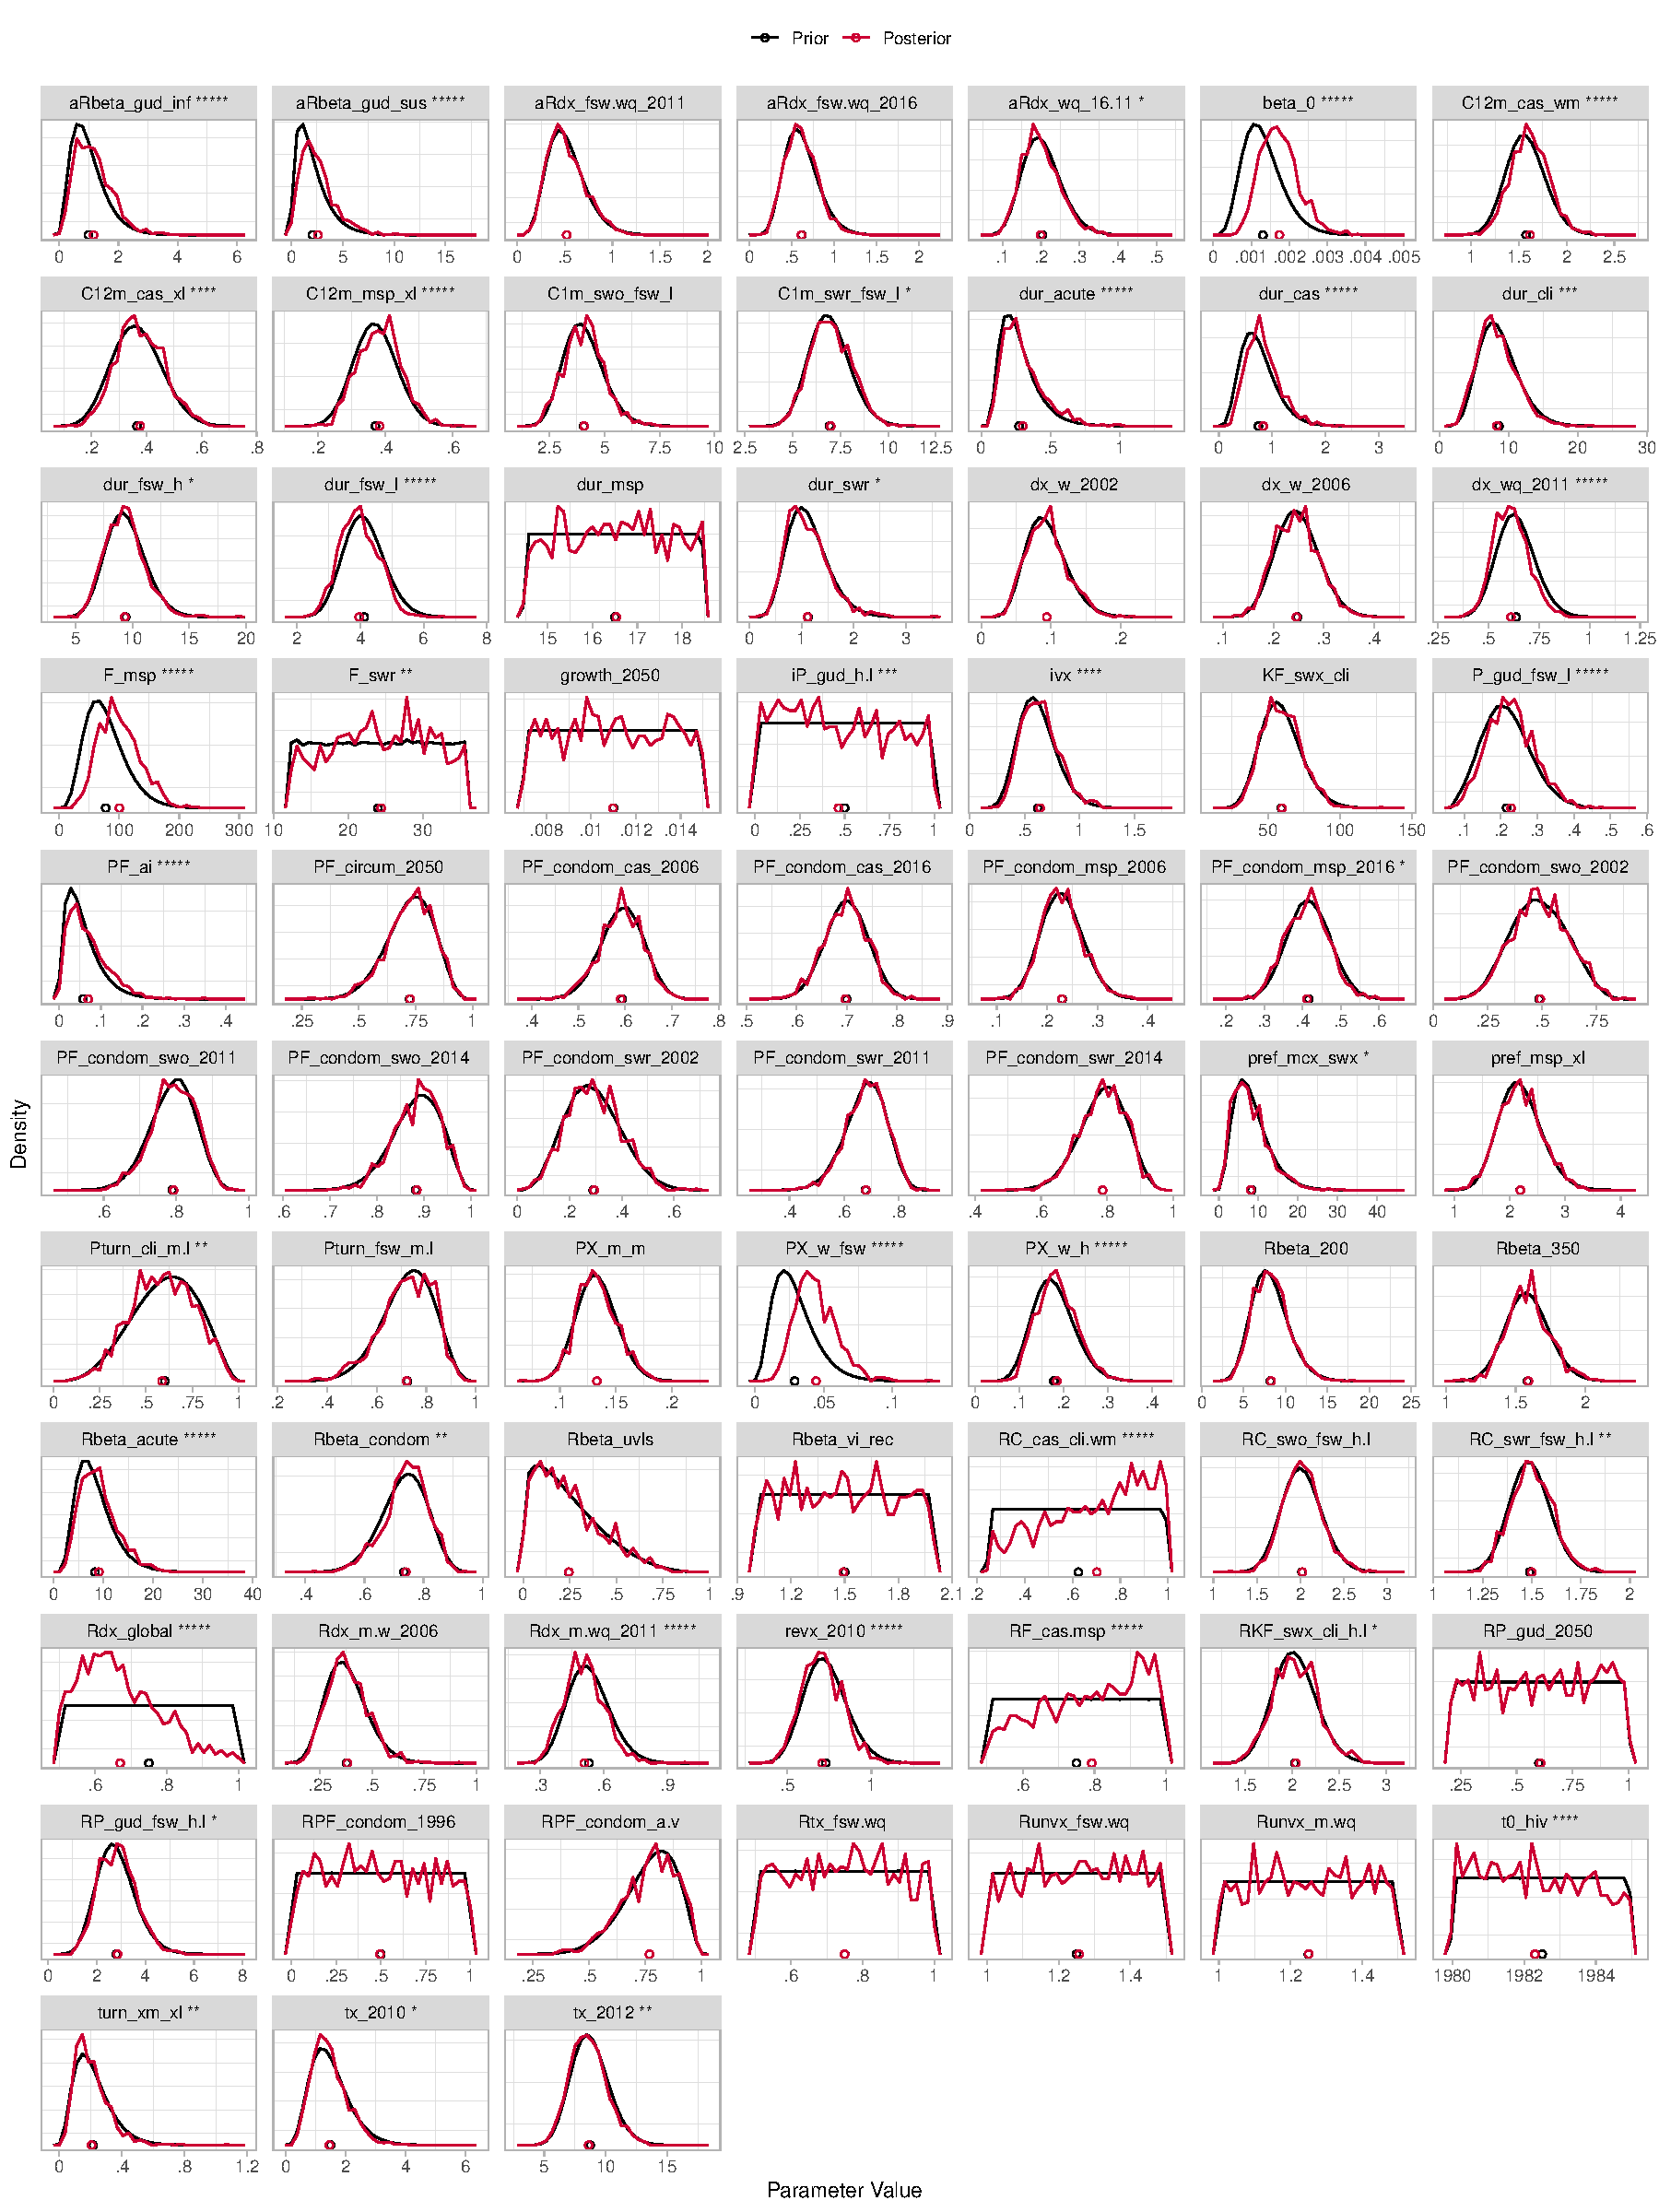
\includegraphics[width=\linewidth]{post.distr}
  \caption{Distributions of calibrated model parameters,
    stratified by prior (all samples) \vs posterior (top 1\% by calibration likelihood)}
  \label{fig:post.distr}
  \floatfoot{
    Asterisks denote significance of Anderson-Darling (AD) Test \cite{Scholz1987}
    for comparing distributions, where $p < 0.1$: *, $p < 0.01$: **, etc;
    see Table~\ref{tab:par.defs} for parameter definitions}
\end{figure}
\par
% MAN
Figure~\ref{fig:post.cor} further illustrates bivariate rank correlations among
posterior parameter values (subset of parameters with at least one correlation $\pm 0.1$).
Of these 18 parameters, 10 were subject to relational constraints (\sref{app.model.cal.constr})
and 10 had highly significant differences between prior and posterior distributions.
For example, condom use levels were \emph{positively} correlated across
regular and occasional sex work partnerships, including over time (\texttt{PF_condom_sw*}), as were
the proportions of anal sex acts in sex work \vs non-sex work partnerships (\texttt{PF_ai_*}).
Multiple combinations of parameters with similar influence on transmission dynamics
were \emph{negatively} correlated, such as
the baseline per-act probability of transmission (\texttt{beta_0}) \vs
relative susceptibility due to GUD (\texttt{aRbeta_gud_sus}), and
diagnosis rates overall (\texttt{Rdx_global}) \vs
among specific risk groups (\texttt{dx_wq_2011}, \texttt{Rdx_m.wq_2011}).
\par
These correlated parameters reflect challenges of non-identifiability \cite{Raue2009},
although no parameters in the model are perfectly non-identifiable.
Thus, the variance of posterior distributions may be inflated for these parameters \cite{Raue2009},
but so long as the joint posterior maintains the observed correlations
--- \ie individual parameter values are not permuted among posterior parameter sets ---
the resulting epidemic simulations should remain plausible.
\begin{figure}
  \centering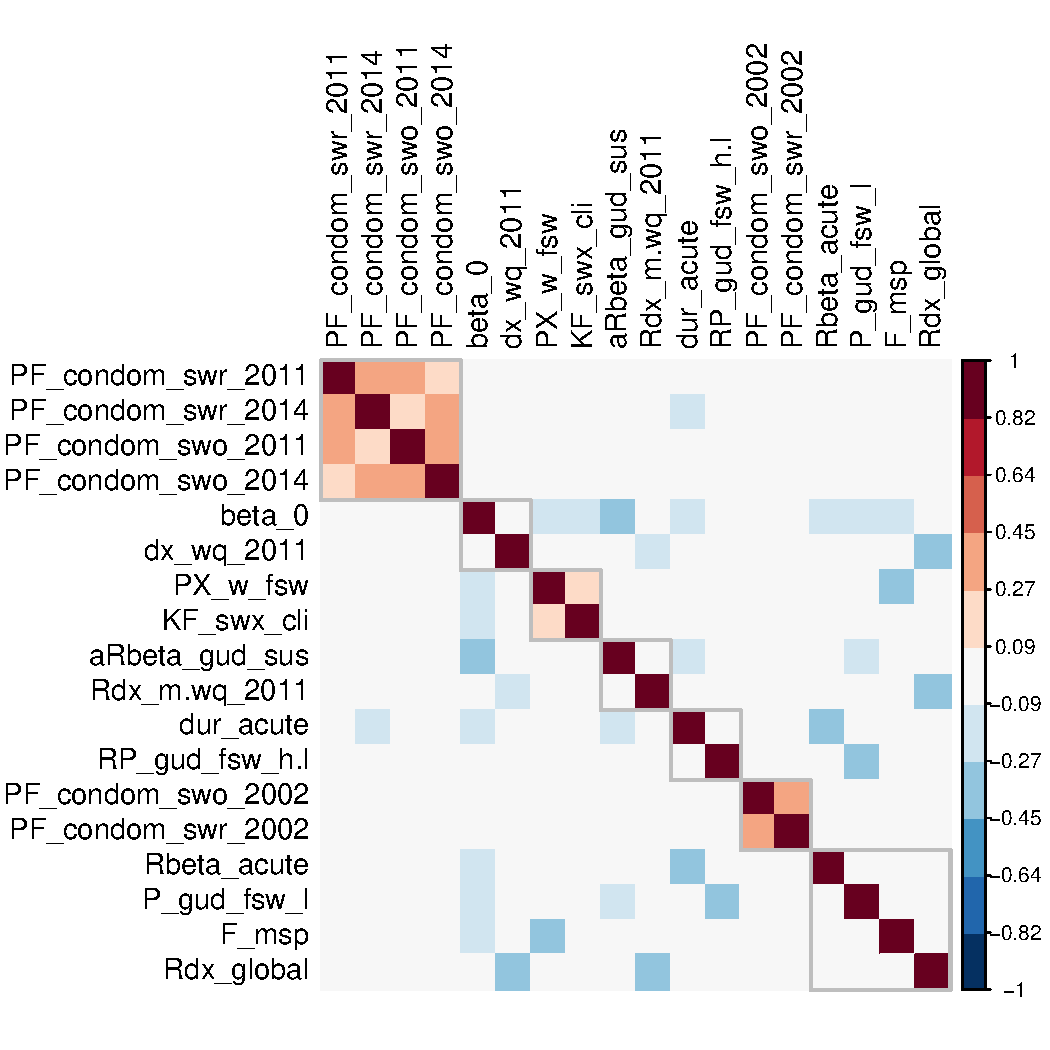
\includegraphics[width=.67\linewidth]{post.cor}
  \caption{Rank correlations among selected posterior model parameters}
  \label{fig:post.cor}
  \floatfoot{
    Subset of parameters with at least one correlation $\pm 0.1$;
    layout computed via hierarchical clustering using the Ward-2 criterion \cite{Murtagh2014};
    gray squares denote computed clusters;
    see Table~\ref{tab:par.defs} for parameter definitions}
\end{figure}
%===================================================================================================
\subsection{Calibration}\label{model.res.cal}
This section presents the estimates of key model outputs
from the 1000 model fits (top 1\% by likelihood among 100,000 sampled parameter sets),
with comparison to the associated calibration targets.
Additional results are given in \sref{app.model.cal.res}, including:
distribution of log-likelihoods (Figure~\ref{fig:fit.ll})
total Eswatini population size aged 15--49 (Figure~\ref{fig:fit.pop}),
and condom use within each partnership type (Figure~\ref{fig:fit.condom}).
%---------------------------------------------------------------------------------------------------
\subsubsection{HIV Prevalence \& Incidence}\label{model.res.cal.hiv}
Figure~\ref{fig:fit.hiv} illustrates the modelled HIV
prevalence \sfref{fig:fit.prev} and incidence \sfref{fig:fit.inc}
among selected risk groups.
Figures \ref{fig:fit.prev1v2}~and~\ref{fig:fit.inc1v2} similarly illustrate
HIV prevalence and incidence ratios, respectively.
Overall, model estimates agree well with the available calibration targets,
with the following shortcomings.
Relative to the calibration targets, the model tends to
underestimate HIV prevalence among women overall,
but overestimate HIV prevalence among men overall, and among FSW prior to 2020.
HIV prevalence and incidence ratios also tend to be overestimated by the model \vs the targets,
with the exception of the prevalence ratio among higher \vs lower risk FSW,
which is reduced towards 1 as prevalence saturates in both groups.
These shortcomings could be explained by
omission of age in the model (see \sref{model.disc.lim.str}) or
insufficient reporting bias adjustment for women's partners ---
despite substantial adjustment in \sref{model.par.wp},
only 18\% of women were modelled to have 2+ partners in p12m, including FSW % MAN
(Figures~\ref{fig:xwp.adj}~and~\ref{fig:xwp.adj.dens}).
Thus, the model may struggle to reproduce high HIV prevalence among women overall,
without high incidence and thus prevalent among FSW and medium activity women.
Indeed, previous work has shown that HIV prevalence among lower risk groups can be
partially driven by turnover of infected individuals from higher risk groups \cite{Knight2020}.
\begin{figure}
  \subcapoverlap
  \foreach \var in {prev,inc}{
    \begin{subfigure}{\linewidth}
      \centering\includegraphics[scale=\fitscale]{fit.\var.base.all}
      \caption{\raggedright}
      \label{fig:fit.\var}
    \end{subfigure}}
  \caption{Modelled HIV prevalence and incidence among selected risk groups
    and associated calibration targets}
  \label{fig:fit.hiv}
  \floatfoot{\fffit; \ffribbon; \ffpbar.}
\end{figure}
\par
Few data are available to validate the modelled early epidemic dynamics.
Modelled incidence among women and men peaked rapidly after introduction of HIV
(Figure~\ref{fig:fit.inc}), corresponding to
rapid acquisition and saturation among higher risk FSW and clients.
Modelled incidence and prevalence continued to increase approximately linearly over 1990--2010,
reflecting a balance of would-be exponential epidemic growth and build-up of mitigating factors,
such as increasing condom use, male circumcision, ART coverage, and
accumulation of seroconcordant partnerships (see \sref{foi.exp.model}).
These trends can be compared with HIV prevalence from Eswatini antenatal care clinics
over the same period (Figure~\ref{fig:fit.prev.anc}), which suggest similar trends.%
\footnote{Antenatal care data were not used as calibration targets because
  such data are known to overestimate HIV prevalence among women overall
  due to non-representative sampling \cite{Gouws2008,Marsh2014}.}
Decline of HIV incidence and prevalence after 2010 can likely be attributed to
rapid ART scale-up (see \sref{model.res.cal.cascade})
and further increases in condom use (Figure~\ref{fig:fit.condom}).
Although modelled incidence declined rapidly, prevalence remained relatively higher
due to increased survival of PLHIV with ART.
In some model fits, prevalence among FSW declined faster than among women overall,
likely due to high turnover of women in sex work.
%---------------------------------------------------------------------------------------------------
\subsubsection{ART Cascade}\label{model.res.cal.cascade}
Figure~\ref{fig:fit.cascade} illustrates the modelled ART cascade among selected risk groups,
including both conditional and unconditional cascade steps,
and the associated calibration targets.
The model estimates agree quite well with these targets, for all risk groups.
The non-monotonic proportions virally suppressed among treated PLHIV
reflect major changes in treatment eligibility (see \sref{model.par.cascade.tx}), which caused
influxes of newly ART-eligible PLHIV to
temporarily decrease the proportions virally suppressed among treated PLHIV.
\begin{figure}
  \subcapoverlap
  \foreach \var in {diag,treat.c,treat.u,vls.c,vls.u}{
  \begin{subfigure}{\linewidth}
    \centering\includegraphics[scale=\fitscale]{fit.\var.base.all}
    \caption{\raggedright}
    \label{fig:fit.\var}
  \end{subfigure}}
  \caption{Modelled ART cascade among selected risk groups
    and associated calibration targets}
  \label{fig:fit.cascade}
  \floatfoot{\ffcas; \fffit; \ffribbon; \ffpbar.}
\end{figure}
%===================================================================================================
\subsection{Who Infected Whom}\label{model.res.wiw}
As further model validation, and to gain insights into the modelled networks of transmission,
this section presents several summaries of ``who infected whom''
--- \ie distributions of yearly infections stratified by
the transmitting group, acquiring group, and partnership type.
Throughout the section, the numbers of yearly infections shown are obtained from
the median value across all 1000 model fits.
\par
Figure~\ref{fig:wiw.base.frto} illustrates
the total numbers and proportions of modelled yearly infections
transmitted from \sfref{fig:wiw.base.from} and
acquired among \sfref{fig:wiw.base.to} modelled risk groups.
Figure~\ref{fig:wiw.base.ratio} then gives
the \emph{ratio} of yearly infections transmitted \vs acquired.
Figure~\ref{fig:wiw.base.part} stratifies yearly infections by partnership type, while
Figure~\ref{fig:wiw.base.alluvial} illustrates
the complete transmission network every 10 years from 1990.
\begin{figure}
  \begin{subfigure}{.5\linewidth}
    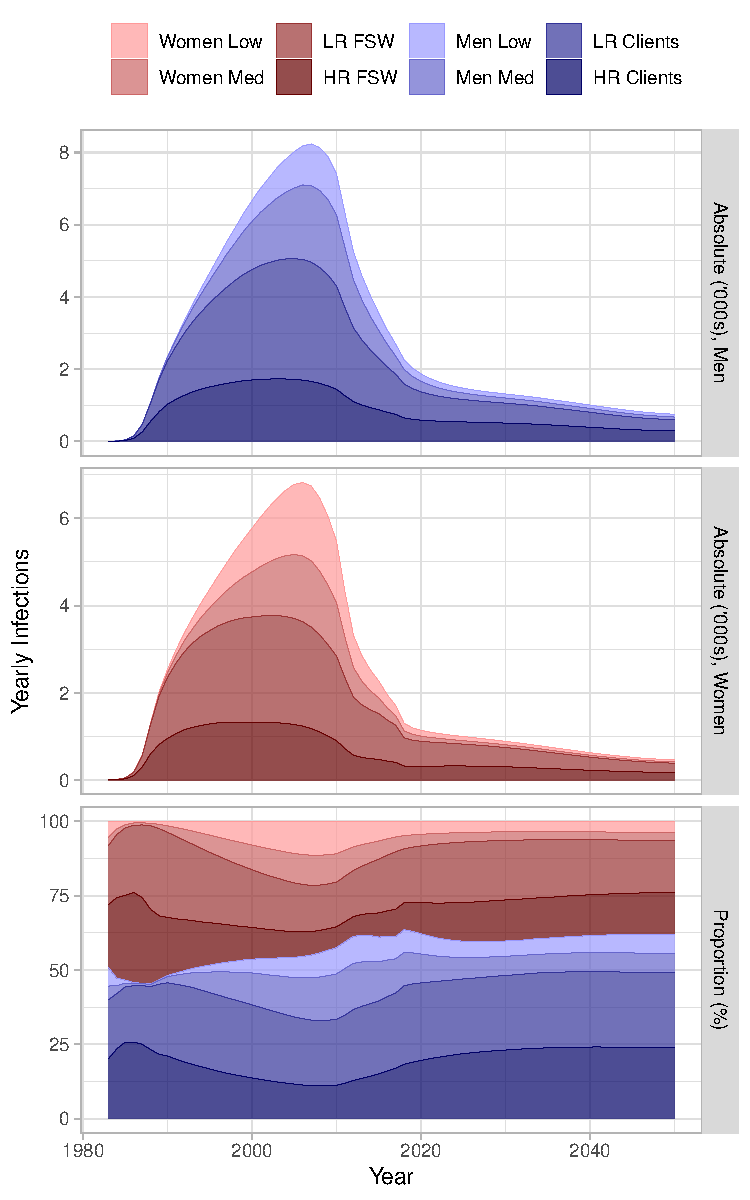
\includegraphics[width=\linewidth]{wiw.base.from}
    \caption{Transmitted from}
    \label{fig:wiw.base.from}
  \end{subfigure}%
  \begin{subfigure}{.5\linewidth}
    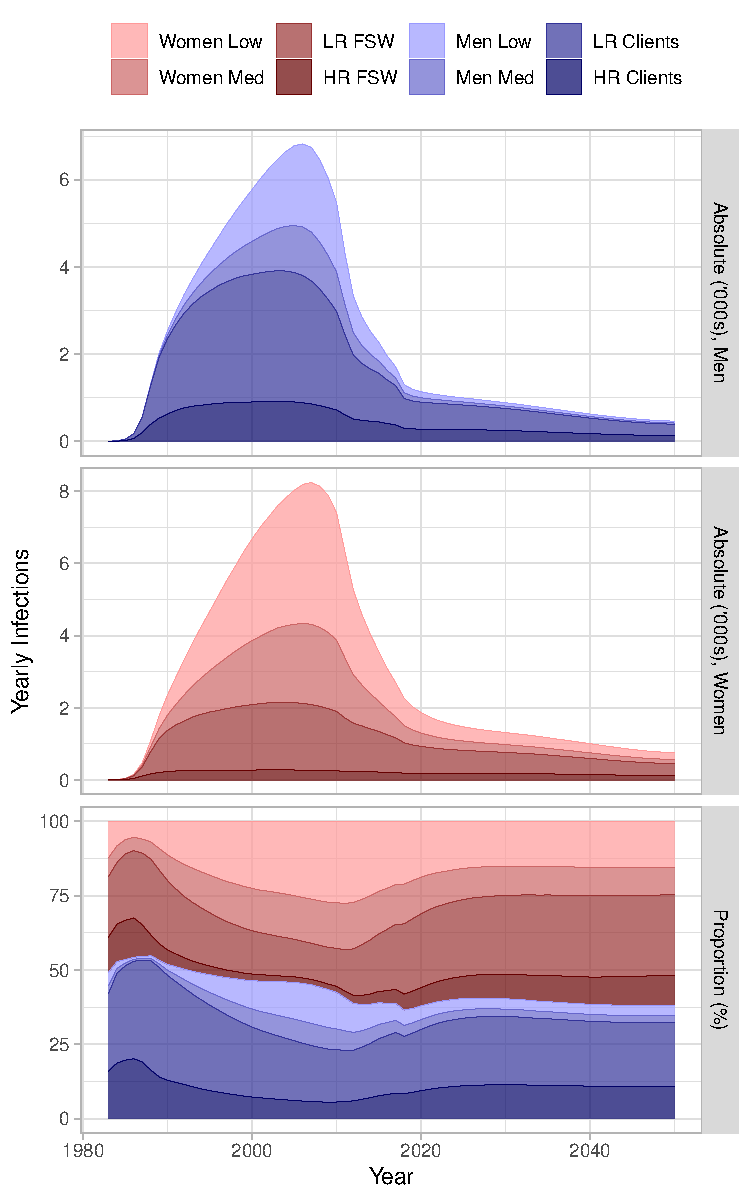
\includegraphics[width=\linewidth]{wiw.base.to}
    \caption{Acquired among}
    \label{fig:wiw.base.to}
  \end{subfigure}
  \caption{Absolute numbers and proportions of modelled yearly HIV infections
    \sfref{fig:wiw.base.from} transmitted from and \sfref{fig:wiw.base.to} acquired among
    risk groups in Eswatini}
  \label{fig:wiw.base.frto}
  \floatfoot{\ffpops; \ffwiw.}
\end{figure}
\begin{figure}
  \begin{minipage}[b]{.49\linewidth}
    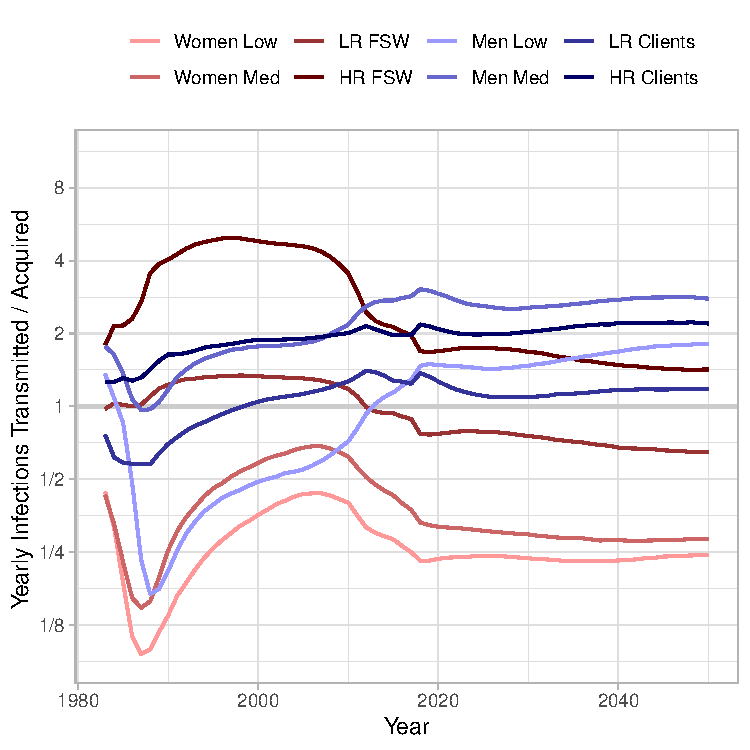
\includegraphics[width=\linewidth]{wiw.base.ratio}
    \caption{Ratio of modelled yearly infections transmitted from \vs acquired among
      risk groups in Eswatini}
    \label{fig:wiw.base.ratio}
  \end{minipage}\hfill
  \begin{minipage}[b]{.49\linewidth}
    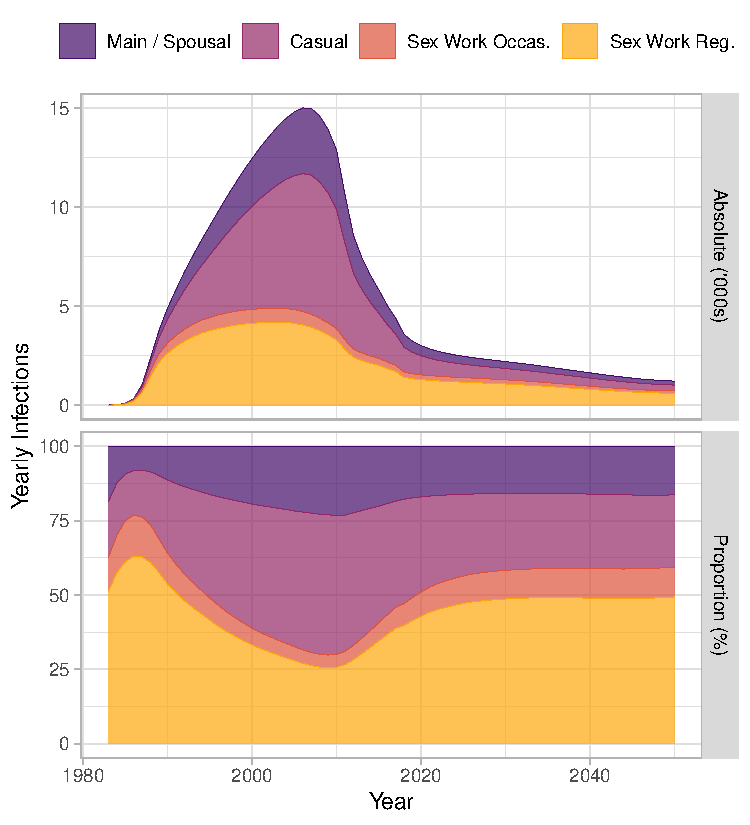
\includegraphics[width=\linewidth]{wiw.base.part}
    \caption{Absolute numbers and proportions of modelled yearly HIV infections
    transmitted via different partnership types in Eswatini}
    \label{fig:wiw.base.part}
  \end{minipage}
  \floatfoot{\ffpops; \ffwiw.}
\end{figure}
\begin{figure}
  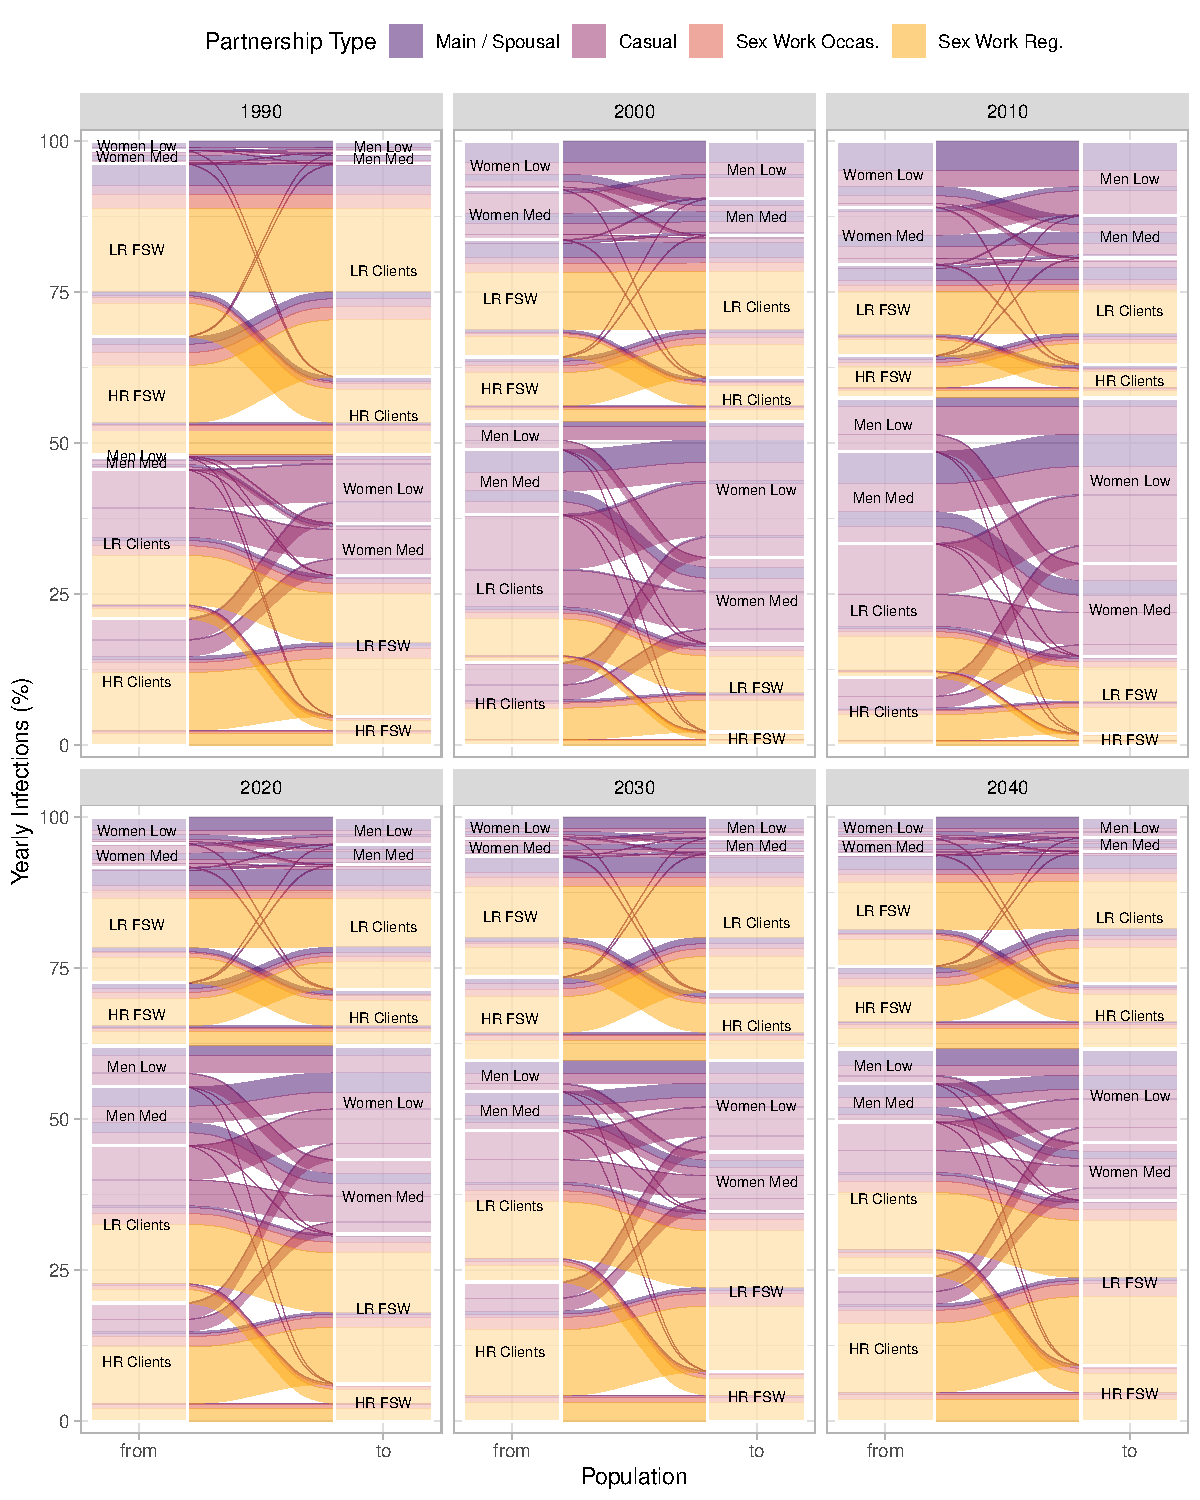
\includegraphics[width=\linewidth]{wiw.base.alluvial}
  \caption{Alluvial diagram showing proportions of all yearly infections (ribbons)
    transmitted from (left) to (right) modelled risk groups,
    stratified by partnership type (color) and year (facets) in Eswatini}
  \label{fig:wiw.base.alluvial}
  \floatfoot{\ffpops; \ffwiw.}
\end{figure}
\par
Before 1990, most infections were transmitted between FSW and their clients,
mainly via regular sex work partnerships.
Indeed, throughout the epidemic, FSW, clients, and regular sex work partnerships
were disproportionately involved in transmission.
Higher risk FSW had the largest ratio of infections transmitted \vs acquired,
suggesting that prevention efforts prioritizing these women
would be highly efficient at reducing overall transmission.
Interestingly, this ratio for lower risk FSW declined and remained below 1
by approximately 2013, % MAN
suggesting that lower risk sex work could be seen as a net sink (\vs source) of new infections,
though the risk of transmission after exiting sex work is not captured by this ratio.
Also, the ratio for medium activity men was sometimes higher than for clients of FSW;
two factors could contribute to this result:
a greater proportion of sexual partners who are susceptible among medium activity men (\ie not FSW),
and greater overall sexual activity \vs lower risk clients in some model fits.
Since many clients are highly mobile for work
and thereby away from regular partners \cite{Carael2006,Matovu2012,Makhakhe2017},
it is not implausible that overall sexual activity could be
lower among some clients \vs a ``medium activity'' group of men.
\par
After 1990, lowest/medium activity women and men began to acquire and transmit
a larger proportion of infections, mainly via casual partnerships,
corresponding with the epidemic peak.
While lowest/medium activity women transmitted similar proportions of infections
\vs lowest/medium activity men,
these women \emph{acquired} substantially more infections than the men,
including projected infections beyond 2020.
As incidence declined over 2010--2020 and beyond,
new infections were modelled to become ``re-concentrated''
within sex work populations and partnerships.
This re-concentration of HIV incidence among higher risk sexual networks
is indeed anticipated across multiple declining epidemics \cite{Brown2019,Ortblad2019},
and likely threatens to undermine the anticipated prevention benefits of ART scale-up
(as explored in Chapter~\ref{art}) \cite{Baral2019}.
